\documentclass[8pt, a4paper, oneside, twocolumn]{extarticle}
\usepackage{graphicx}
\usepackage[export]{adjustbox}
\usepackage[compact]{titlesec}  % documentation: http://mirror.iopb.res.in/tex-archive/macros/latex/contrib/titlesec/titlesec.pdf  
\usepackage{kotex}
\usepackage[left=0.8cm, right=0.8cm, top=2cm, bottom=0.3cm, a4paper]{geometry}
\usepackage{amsmath}
\usepackage{ulem}
\usepackage{amssymb}
\usepackage{minted}  % syntax highlighting
\usepackage{enumitem}
\setlist{nolistsep}
\usepackage{fancyhdr} % documentation: http://ctan.math.utah.edu/ctan/tex-archive/macros/latex/contrib/fancyhdr/fancyhdr.pdf
\usepackage{lastpage}  % just so that we can use \pageref {LastPage}
\usepackage{color, hyperref}
% The lines in the table of contents become links to the corresponding pages in the document by simply adding in the preamble of the document the line
\usepackage{tikz}
\usetikzlibrary{positioning,chains,fit,shapes,calc}
\newcommand{\swastik}[1]{%
    \begin{tikzpicture}[#1]
        \draw (-1,1)  -- (-1,0) -- (1,0) -- (1,-1);
        \draw (-1,-1) -- (0,-1) -- (0,1) -- (1,1);
    \end{tikzpicture}%
}
\newcommand{\revised}{To be \textcolor{red}{\textbf{revised}}.}
\titlespacing*{\section}
{0pt}{0px plus 1px minus 0px}{-2px plus 0px minus 0px}
\titlespacing*{\subsection}
{0pt}{0px plus 1px minus 0px}{0px plus 3px minus 3px}
\titlespacing*{\subsubsection}
{0pt}{0px plus 1px minus 0px}{0px plus 3px minus 3px}
\setlength{\columnseprule}{0.4pt}
\DeclareRobustCommand{\stirling}{\genfrac\{\}{0pt}{}}
\setlength{\parindent}{0pt}  % so that there is no indent of paras.
\setminted{breaklines=true, tabsize=2, breaksymbolleft=}
\begin{document}
\pagenumbering{arabic}
\title{\swastik {scale = 0.2} {}DBMS Short Revision Notes{} \swastik {scale = 0.2}}
\author{Sourabh Aggarwal}
\date{Compiled on \today}
\maketitle
\tableofcontents
\thispagestyle{fancy}  % else it was not giving fancy header to the first page
\newpage
\section{Intro}
Database is simply a collection of related info.

Create Read (Retrieve) Update Delete (CRUD)

Two types of Databases:-
\begin{itemize}
\item Relational Databases (SQL): Organize data into one or more tables, each table has columns and rows and a unique key identifies each row.
\item Non Relational (noSQL / not just SQL): Organize data is anything but a traditional table. Like key value stores, Documents (JSON), Graphs, etc.
\end{itemize}
Relational database management systems (RDBMS): softwares which help users create and maintain a a relational database. Ex: mySQL

Schema: Is just an overall structure of our database, columns, their types etc.

SQL (Standard Query Language): Standardized language for interacting with RDBMS. It's basically 4 types of languages in one: 
\begin{itemize}
    \item Data Query Language (DQL)
    \item Data Definition Language (schemas etc.)
    \item Data Control Language (permissions etc.)
    \item Data Manipulation Language (update etc.)
\end{itemize}

Queries are requests made to the database management systems for specific information.

Primary Key: Column which uniquely identifies each row. (It cannot contain NULL values.) Tables are limited to ONE primary key each.

Surrogate key: Primary key which has no inference, just a random no.

Natural Key: Aadhaar no., etc. which have real world inference/mapping. (it is a primary key)

Composite Key: Key which requires 2 or more attributes, Primary key can be a composite key. 

Foreign Key: Attribute which will link us to another database table. Foreign key stores primary key of a row of another database table. A particular table can have more than one foreign key. And it can have NULL values. Primary key could be a composite of foreign keys.

Code written
\begin{minted}{SQL}
create database girrafe;

INT -- whole numbers
DECIMAL(M, N) -- M is the total no. of digits and N is the no. of digits after the decimal point.
VALCHAR(l) -- String of length l.
BLOB -- Binary Large Object
DATE -- 'YYYY-MM-DD'
TIMESTAMP -- 'YYYY-MM-DD HH:MM:SS'


CREATE TABLE student (
    student_id INT PRIMARY KEY,
    name VARCHAR (30),
    major VARCHAR (20)
);

DESCRIBE student;  -- Describes our table

DROP TABLE student;  -- Deletes our table

ALTER TABLE student ADD gpa DECIMAL (3, 2);  -- Add a column to our table

ALTER TABLE student DROP COLUMN gpa;  -- drops our gpa column

SELECT * FROM student;  -- show all rows


INSERT INTO student VALUES (1, 'Jack', 'Biology');  -- add this row, parameters should be given in order

INSERT INTO student (student_id, name) VALUES (2, 'Kate');  -- Now we need not include 'major', it will show 'NULL' in major now.
\end{minted}
\begin{minted}{SQL}
UPDATE student
SET major = 'Bio'
WHERE major = 'Biology';  -- other operators are <> (not equal), > (greater), <, >=, <=. our target is to update the major name to Bio in case the major name is Biology
-- Or we could have done WHERE student_id > 3;
-- Or SET major = 'Biochemistry'
-- WHERE major = 'Bio' OR major = 'Chemistry';
-- SET name = 'Tom', major = 'undecided'
-- WHERE student_id = 1;
-- Note: If we remove WHERE then it will affect all of the rows.
DELETE FROM student -- if we put semicolon at the end of this statement then it will delete all of the rows in the table
WHERE name = 'Tom' AND major = 'undecided';
------------------
SELECT name, major
FROM student;  -- now we will get only two columns name, major
--
SELECT name, major
FROM student
ORDER by name DESC; -- will give the entries in the descending order of names. If we remove DESC then it will be order by ascending order. btw ASC can as well be used instead.
-- ORDER by major, student_id DESC; -- will order by major and in case there is a tie then they will be ordered by descending student_id.
-- We can add LIMIT 2; this would give us only 2 entries.
SELECT name, major
FROM student
WHERE name IN ('Claire', 'Kate', 'Mike') AND student_id > 2; -- IN checks for set membership
\end{minted}
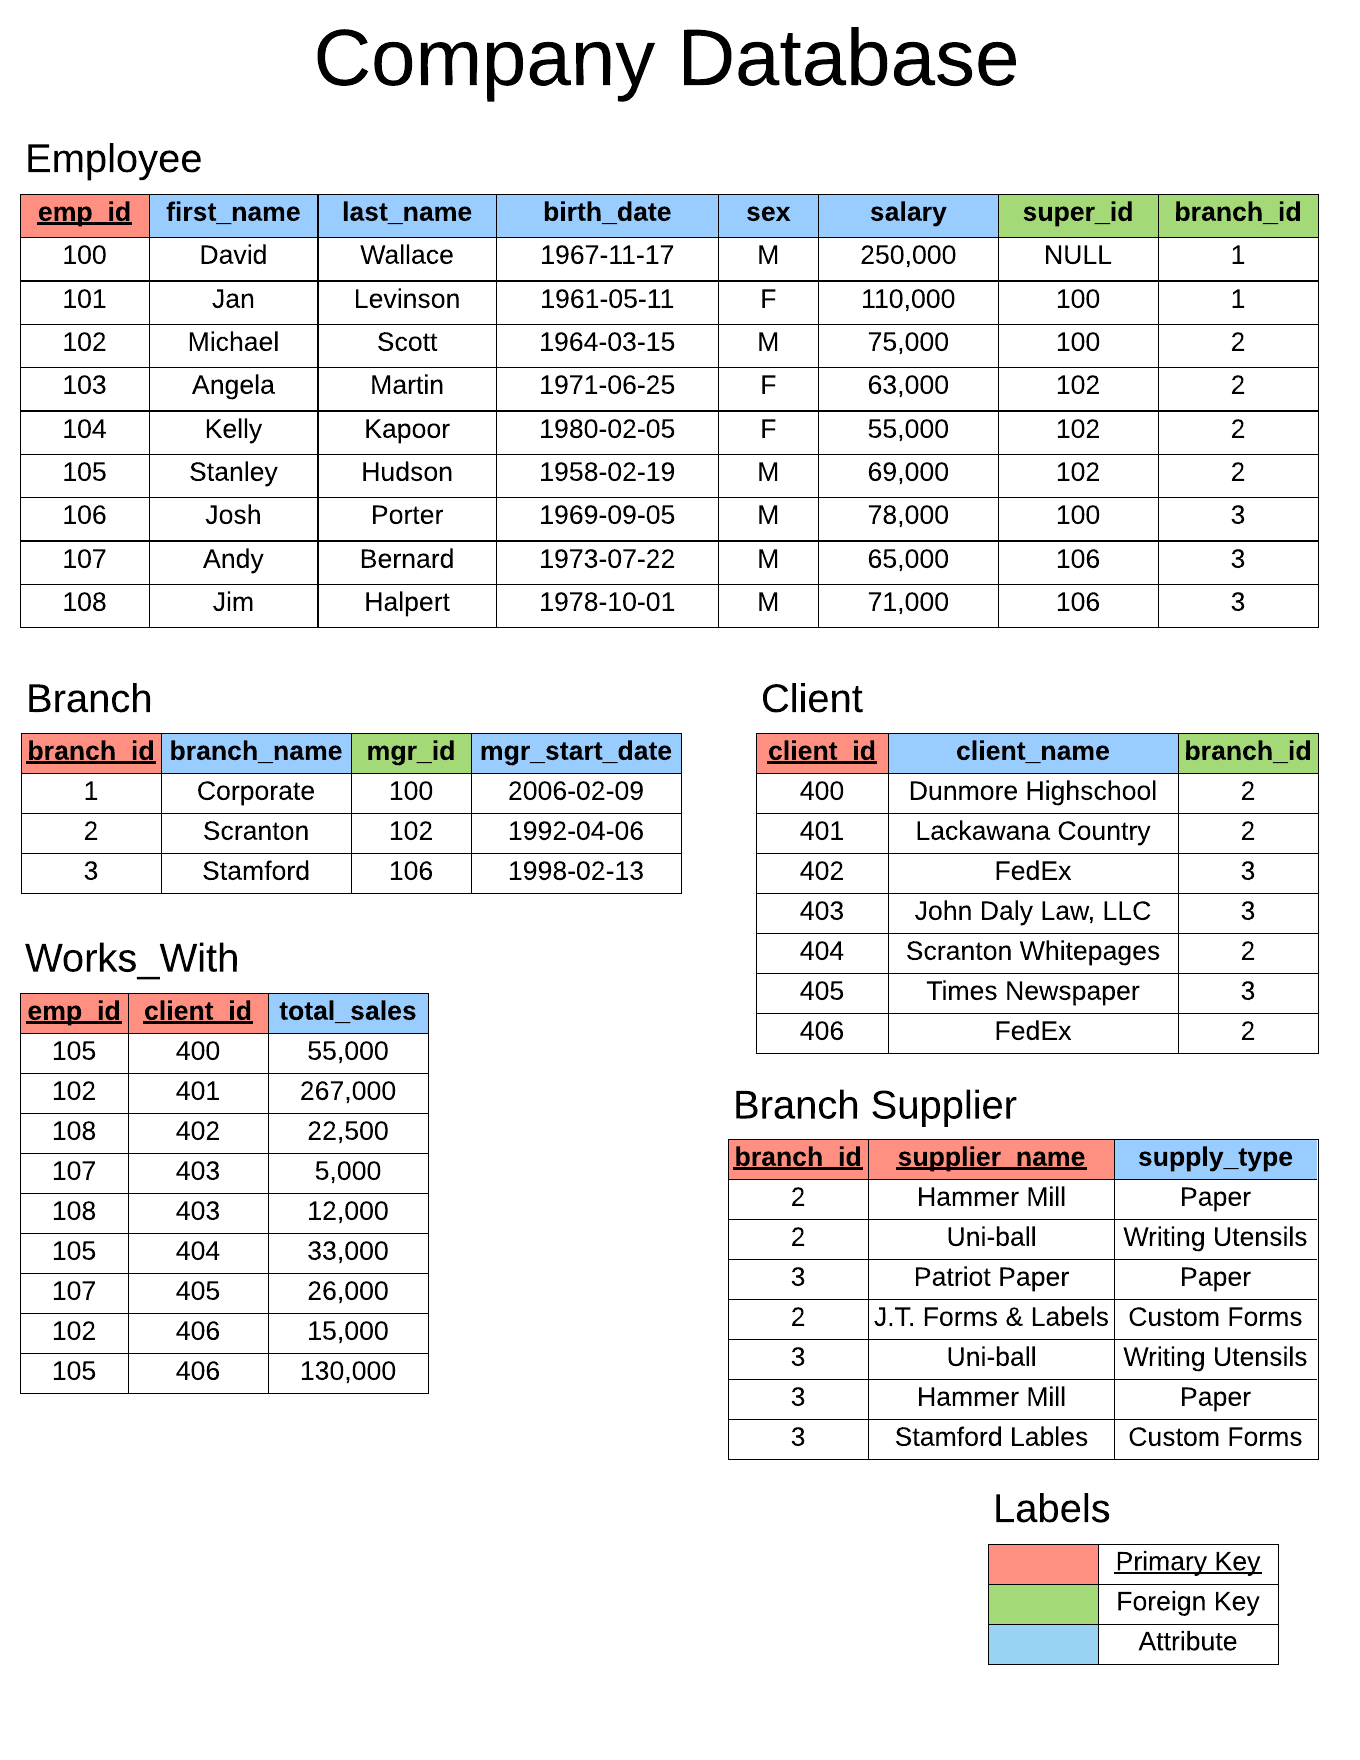
\includegraphics[width=0.5\textwidth,height=0.5\textheight,keepaspectratio]{company-database}
\begin{minted}{SQL}
CREATE TABLE employee (
  emp_id INT PRIMARY KEY,
  first_name VARCHAR(40),
  last_name VARCHAR(40),
  birth_day DATE,
  sex VARCHAR(1),
  salary INT,
  super_id INT,
  branch_id INT
);

CREATE TABLE branch (
  branch_id INT PRIMARY KEY,
  branch_name VARCHAR(40),
  mgr_id INT,
  mgr_start_date DATE,
  FOREIGN KEY(mgr_id) REFERENCES employee(emp_id) ON DELETE SET NULL
);

ALTER TABLE employee
ADD FOREIGN KEY(branch_id)
REFERENCES branch(branch_id)
ON DELETE SET NULL;

ALTER TABLE employee
ADD FOREIGN KEY(super_id)
REFERENCES employee(emp_id)
ON DELETE SET NULL;

CREATE TABLE client (
  client_id INT PRIMARY KEY,
  client_name VARCHAR(40),
  branch_id INT,
  FOREIGN KEY(branch_id) REFERENCES branch(branch_id) ON DELETE SET NULL
);

CREATE TABLE works_with (
  emp_id INT,
  client_id INT,
  total_sales INT,
  PRIMARY KEY(emp_id, client_id),
  FOREIGN KEY(emp_id) REFERENCES employee(emp_id) ON DELETE CASCADE,
  FOREIGN KEY(client_id) REFERENCES client(client_id) ON DELETE CASCADE
);

CREATE TABLE branch_supplier (
  branch_id INT,
  supplier_name VARCHAR(40),
  supply_type VARCHAR(40),
  PRIMARY KEY(branch_id, supplier_name),
  FOREIGN KEY(branch_id) REFERENCES branch(branch_id) ON DELETE CASCADE
);


-- -----------------------------------------------------------------------------

-- Corporate
INSERT INTO employee VALUES(100, 'David', 'Wallace', '1967-11-17', 'M', 250000, NULL, NULL);

INSERT INTO branch VALUES(1, 'Corporate', 100, '2006-02-09');

UPDATE employee
SET branch_id = 1
WHERE emp_id = 100;

INSERT INTO employee VALUES(101, 'Jan', 'Levinson', '1961-05-11', 'F', 110000, 100, 1);

-- Scranton
INSERT INTO employee VALUES(102, 'Michael', 'Scott', '1964-03-15', 'M', 75000, 100, NULL);

INSERT INTO branch VALUES(2, 'Scranton', 102, '1992-04-06');

UPDATE employee
SET branch_id = 2
WHERE emp_id = 102;

INSERT INTO employee VALUES(103, 'Angela', 'Martin', '1971-06-25', 'F', 63000, 102, 2);
INSERT INTO employee VALUES(104, 'Kelly', 'Kapoor', '1980-02-05', 'F', 55000, 102, 2);
INSERT INTO employee VALUES(105, 'Stanley', 'Hudson', '1958-02-19', 'M', 69000, 102, 2);

-- Stamford
INSERT INTO employee VALUES(106, 'Josh', 'Porter', '1969-09-05', 'M', 78000, 100, NULL);

INSERT INTO branch VALUES(3, 'Stamford', 106, '1998-02-13');

UPDATE employee
SET branch_id = 3
WHERE emp_id = 106;

INSERT INTO employee VALUES(107, 'Andy', 'Bernard', '1973-07-22', 'M', 65000, 106, 3);
INSERT INTO employee VALUES(108, 'Jim', 'Halpert', '1978-10-01', 'M', 71000, 106, 3);


-- BRANCH SUPPLIER
INSERT INTO branch_supplier VALUES(2, 'Hammer Mill', 'Paper');
INSERT INTO branch_supplier VALUES(2, 'Uni-ball', 'Writing Utensils');
INSERT INTO branch_supplier VALUES(3, 'Patriot Paper', 'Paper');
INSERT INTO branch_supplier VALUES(2, 'J.T. Forms & Labels', 'Custom Forms');
INSERT INTO branch_supplier VALUES(3, 'Uni-ball', 'Writing Utensils');
INSERT INTO branch_supplier VALUES(3, 'Hammer Mill', 'Paper');
INSERT INTO branch_supplier VALUES(3, 'Stamford Lables', 'Custom Forms');

-- CLIENT
INSERT INTO client VALUES(400, 'Dunmore Highschool', 2);
INSERT INTO client VALUES(401, 'Lackawana Country', 2);
INSERT INTO client VALUES(402, 'FedEx', 3);
INSERT INTO client VALUES(403, 'John Daly Law, LLC', 3);
INSERT INTO client VALUES(404, 'Scranton Whitepages', 2);
INSERT INTO client VALUES(405, 'Times Newspaper', 3);
INSERT INTO client VALUES(406, 'FedEx', 2);

-- WORKS_WITH
INSERT INTO works_with VALUES(105, 400, 55000);
INSERT INTO works_with VALUES(102, 401, 267000);
INSERT INTO works_with VALUES(108, 402, 22500);
INSERT INTO works_with VALUES(107, 403, 5000);
INSERT INTO works_with VALUES(108, 403, 12000);
INSERT INTO works_with VALUES(105, 404, 33000);
INSERT INTO works_with VALUES(107, 405, 26000);
INSERT INTO works_with VALUES(102, 406, 15000);
INSERT INTO works_with VALUES(105, 406, 130000);

-- Find all employees
SELECT *
FROM employee;

-- Find all clients
SELECT *
FROM clients;

-- Find all employees ordered by salary
SELECT *
from employee
ORDER BY salary ASC/DESC;

-- Find all employees ordered by sex then name
SELECT *
from employee
ORDER BY sex, name;

-- Find the first 5 employees in the table
SELECT *
from employee
LIMIT 5;

-- Find the first and last names of all employees
SELECT first_name, employee.last_name
FROM employee;

-- Find the forename and surnames names of all employees
SELECT first_name AS forename, employee.last_name AS surname
FROM employee;

-- Find out all the different genders
SELECT DISCINCT sex
FROM employee;

-- Find all male employees
SELECT *
FROM employee
WHERE sex = 'M';

-- Find all employees at branch 2
SELECT *
FROM employee
WHERE branch_id = 2;

-- Find all employee's id's and names who were born after 1969
SELECT emp_id, first_name, last_name
FROM employee
WHERE birth_day >= 1970-01-01;

-- Find all female employees at branch 2
SELECT *
FROM employee
WHERE branch_id = 2 AND sex = 'F';

-- Find all employees who are female & born after 1969 or who make over 80000
SELECT *
FROM employee
WHERE (birth_day >= '1970-01-01' AND sex = 'F') OR salary > 80000;

-- Find all employees born between 1970 and 1975
SELECT *
FROM employee
WHERE birth_day BETWEEN '1970-01-01' AND '1975-01-01';

-- Find all employees named Jim, Michael, Johnny or David
SELECT *
FROM employee
WHERE first_name IN ('Jim', 'Michael', 'Johnny', 'David');

-- Functions

-- Find the number of employees
SELECT COUNT(super_id)
FROM employee;

-- Find the average of all employee's salaries
SELECT AVG(salary)
FROM employee;

-- Find the sum of all employee's salaries
SELECT SUM(salary)
FROM employee;

-- Aggregation.
-- Find out how many males and females there are
SELECT COUNT(sex), sex
FROM employee
GROUP BY sex

-- Find the total sales of each salesman
SELECT SUM(total_sales), emp_id
FROM works_with
GROUP BY client_id;

-- Find the total amount of money spent by each client
SELECT SUM(total_sales), client_id
FROM works_with
GROUP BY client_id;

-- Wildcards

-- % = any # characters, _ = one character

-- Find any client's who are an LLC
SELECT *
FROM client
WHERE client_name LIKE '%LLC';

-- Find any branch suppliers who are in the label business
SELECT *
FROM branch_supplier
WHERE supplier_name LIKE '% Label%';

-- Find any employee born on the 10th day of the month
SELECT *
FROM employee
WHERE birth_day LIKE '_____10%';

-- Find any clients who are schools
SELECT *
FROM client
WHERE client_name LIKE '%Highschool%';

-- Union

-- Find a list of employee and branch names
SELECT employee.first_name AS Employee_Branch_Names
FROM employee
UNION
SELECT branch.branch_name
FROM branch;

-- Find a list of all clients & branch suppliers' names
SELECT client.client_name AS Non-Employee_Entities, client.branch_id AS Branch_ID
FROM client
UNION -- both above and below thing should have same number of columns and same data type respectively
SELECT branch_supplier.supplier_name, branch_supplier.branch_id
FROM branch_supplier;

-- JOINS (used to combine rows from two or more tables based on the related columns)

-- Add the extra branch
INSERT INTO branch VALUES(4, "Buffalo", NULL, NULL);

-- Find all branches and the names of their managers
SELECT employee.emp_id, employee.first_name, branch.branch_name
FROM employee
JOIN branch    -- LEFT JOIN (when we use LEFT JOIN all the rows from the left table gets included as well, similarly for RIGHT JOIN), RIGHT JOIN  (we added buffalo just so that we can see difference in case of RIGHT JOIN)
ON employee.emp_id = branch.mgr_id;

-- nested queries

-- Find names of all employees who have sold over 50,000
SELECT employee.first_name, employee.last_name
FROM employee
WHERE employee.emp_id IN (SELECT works_with.emp_id  -- note that first sql will execute the part which is inside "()"
                          FROM works_with
                          WHERE works_with.total_sales > 50000);

-- Find all clients who are handles by the branch that Michael Scott manages
-- Assume you know Michael's ID
SELECT client.client_id, client.client_name
FROM client
WHERE client.branch_id = (SELECT branch.branch_id
                          FROM branch
                          WHERE branch.mgr_id = 102);

 -- Find all clients who are handles by the branch that Michael Scott manages
 -- Assume you DONT'T know Michael's ID
 SELECT client.client_id, client.client_name
 FROM client
 WHERE client.branch_id = (SELECT branch.branch_id
                           FROM branch
                           WHERE branch.mgr_id = (SELECT employee.emp_id
                                                  FROM employee
                                                  WHERE employee.first_name = 'Michael' AND employee.last_name ='Scott'
                                                  LIMIT 1));


-- Find the names of employees who work with clients handled by the scranton branch
SELECT employee.first_name, employee.last_name
FROM employee
WHERE employee.emp_id IN (
                         SELECT works_with.emp_id
                         FROM works_with
                         )
AND employee.branch_id = 2;

-- Find the names of all clients who have spent more than 100,000 dollars
SELECT client.client_name
FROM client
WHERE client.client_id IN (
                          SELECT client_id
                          FROM (
                                SELECT SUM(works_with.total_sales) AS totals, client_id
                                FROM works_with
                                GROUP BY client_id) AS total_client_sales
                          WHERE totals > 100000
);

-- deleting entries in the table when they have foreign keys associated to them
-- ON DELETE NULL means that say if we delete Michael Scott then second entry in the branch table will get mgr_id set to NULL whereas in ON DELETE CASCADE the entire row will get deleted in branch table. Use ON DELETE CASCADE when that foreign key is very important like say it forms a primary key.


-- CREATE
--     TRIGGER `event_name` BEFORE/AFTER INSERT/UPDATE/DELETE
--     ON `database`.`table`
--     FOR EACH ROW BEGIN
-- 		-- trigger body
-- 		-- this code is applied to every
-- 		-- inserted/updated/deleted row
--     END;

CREATE TABLE trigger_test (
     message VARCHAR(100)
);


DELIMITER $$  -- changing delimiter from semicolon to $$ as we will be using semicolon inside and we don't want sql to think that when we put semicolon we are done with our trigger
CREATE
    TRIGGER my_trigger BEFORE INSERT
    ON employee
    FOR EACH ROW BEGIN  -- for each new item that is inserted
        INSERT INTO trigger_test VALUES('added new employee');
    END$$
DELIMITER ;  -- changing delimiter back to semi colon.
INSERT INTO employee
VALUES(109, 'Oscar', 'Martinez', '1968-02-19', 'M', 69000, 106, 3);


DELIMITER $$
CREATE
    TRIGGER my_trigger BEFORE INSERT
    ON employee
    FOR EACH ROW BEGIN
        INSERT INTO trigger_test VALUES(NEW.first_name);
    END$$
DELIMITER ;
INSERT INTO employee
VALUES(110, 'Kevin', 'Malone', '1978-02-19', 'M', 69000, 106, 3);

DELIMITER $$
CREATE
    TRIGGER my_trigger BEFORE INSERT
    ON employee
    FOR EACH ROW BEGIN 
         IF NEW.sex = 'M' THEN
               INSERT INTO trigger_test VALUES('added male employee');
         ELSEIF NEW.sex = 'F' THEN
               INSERT INTO trigger_test VALUES('added female');
         ELSE
               INSERT INTO trigger_test VALUES('added other employee');
         END IF;
    END$$
DELIMITER ;
INSERT INTO employee
VALUES(111, 'Pam', 'Beesly', '1988-02-19', 'F', 69000, 106, 3);


DROP TRIGGER my_trigger;
\end{minted}
Entity = An object we want to model and store information about
Attributes = Specific pieces of information about an entity
Composite attribute = An attribute that can be broken up into sub attributes
Multi - valued attribute = An attribute than can have more than one value (like same student can have more than one club but only one GPA)
Derived Attribute = An attribute that can be derived from the other attributes.
ER = Entity Relationship defines a relationship between two entities.
Relationship Attribute = An attribute about the relationship

\end{document}